\documentclass{article}
\usepackage[T1]{fontenc}
\usepackage{lmodern}
\usepackage{graphicx}
\usepackage{amsmath,amssymb}
\usepackage[a4paper,margin=2cm]{geometry}
\usepackage[absolute,overlay]{textpos}
\setlength{\TPHorizModule}{1mm}
\setlength{\TPVertModule}{1mm}
\usepackage[indonesian]{babel}
\usepackage{hyperref}
\setlength{\emergencystretch}{2em}
% unit: Halaman 117

\begin{document}

% === Halaman 117 (llm) ===

\vspace{214.14mm}

Plaintext:\\
PESAW ATMEN DARAT\\\vspace{5mm}
Ciphertext:\\
GUFYL FRKQE JXVHM

% deskripsi: Simulasi mesin Enigma yang menunjukkan keyboard, panel lampu indikator huruf, dan output teks plaintext serta ciphertext.
% bbox normalisasi: [0.3030, 0.1330, 0.6700, 0.8540]
\begin{textblock*}{77.07mm}(63.63mm,39.50mm)
\noindent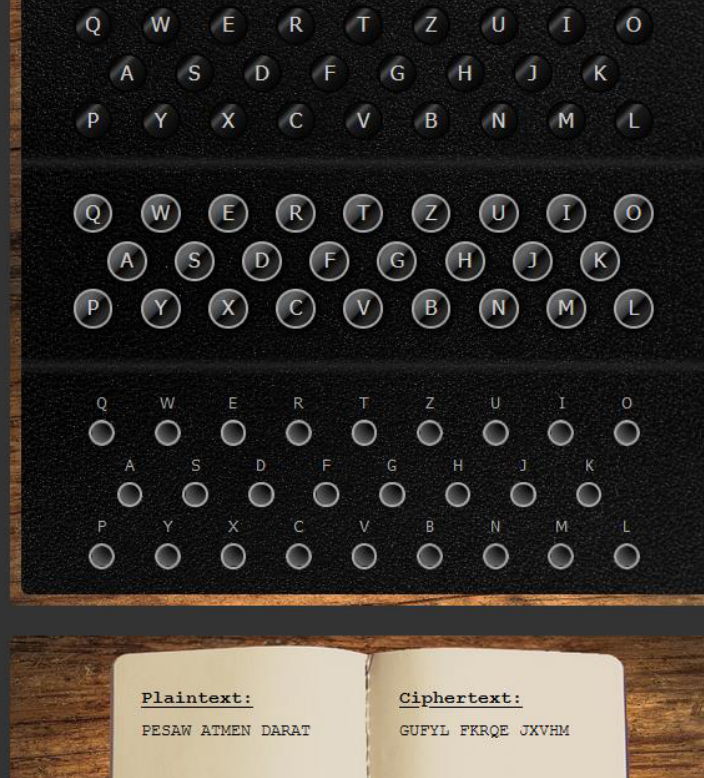
\includegraphics[width=77.07mm,height=214.14mm]{../../images/llm/page_117_img_01.png}%
\end{textblock*}

\end{document}
